\Exercise El vector $\overrightarrow{PQ}=(-4,8)$ té l'origen en el punt $P(6,-1)$. Determina les coordinades de l'extrem $Q$ i el mòdul d'aquest vector.

\Answer

Podem expressar el vector $\overrightarrow{PQ}$ com la diferència dels vectors que identifiquen els seus dos extrems:

\begin{minipage}{0.49\linewidth}
  \[\overrightarrow{PQ}=Q-P\]
\begin{eqnarray*}
  (-4,8)&=&Q-(6,-1)\\
  (-4,8)+(6,-1)&=&Q\\
  (2,7)&=&Q
\end{eqnarray*}
Pel que fa al mòdul:
\[\abs{\overrightarrow{PQ}}=\sqrt{(-4)^2+8^2}=\sqrt{80}=4\sqrt{5}\]
\end{minipage}
\hspace{0.01\linewidth}
\begin{minipage}{0.49\linewidth}
\begin{center}
  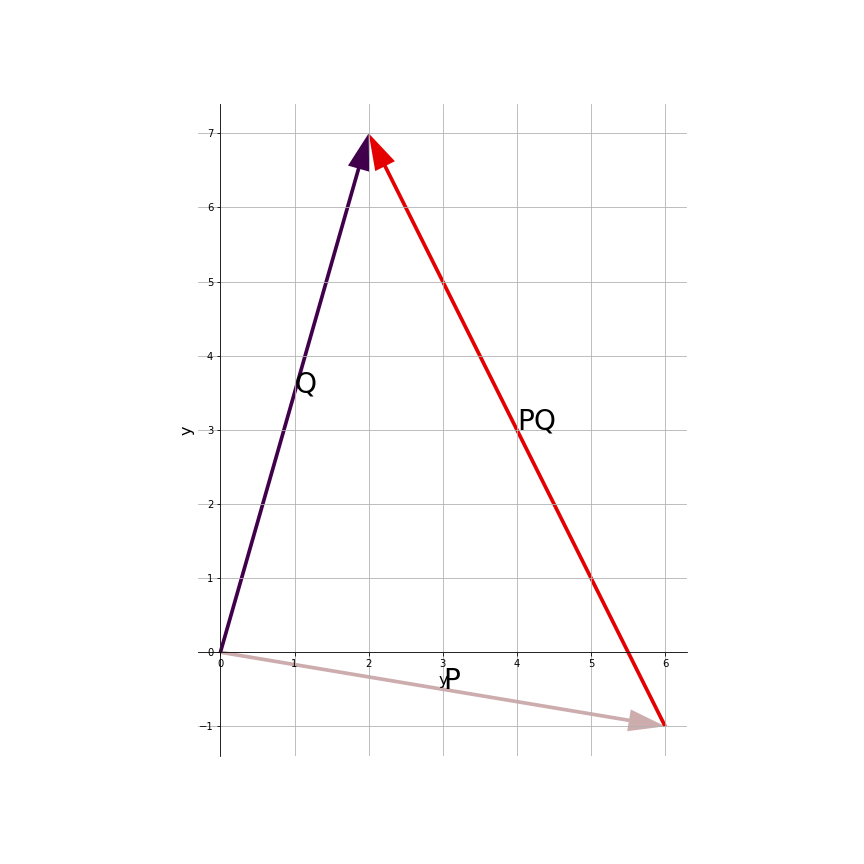
\includegraphics[scale=0.3]{vectorPQ}
\end{center}
\end{minipage}


\blacksquare 